\documentclass{article}
\usepackage{amsmath}
\usepackage{longtable}
\usepackage{csvsimple}
\usepackage{graphicx}

\title{COMP 424 - Artificial Intelligence - Homework \#1}
\author{Kevin Li - 260565522}
\date{Jan 21, 2016}
\begin{document}
\maketitle
\newpage

\section{Question 1 - Search}
\begin{enumerate}
\item % Part 1a
    \begin{description}
        \item[Breadth First Search] Gare du Nord, Rogier, Yser,
            Ribaucourt, Simonis, Belgica, Pannenhuis, Bockstael,
            Stuybenbergh, Houba-Brugmann, Heysel, Roi Baudouin

        \item[Uniform Cost Search] Same as BFS given that all
            operators have unit costs.
            (Gare du Nord, Rogier, Yser, Ribaucourt, Simonis, Belgica, Pannenhuis, Bockstael, Stuybenbergh, Houba-Brugmann, Heysel, Roi Baudouin)

        \item[Depth First Search] Gare du Nord, Rogier, Botanique, Madou, Arts-Loi, Trone, Porte de Namur, Louise, Hotel des Monnaies, Porte de Hal, Gare du Midi, Clemenceau, Delacroix, Gare de l'Ouest, Beekkant, Osseghem, Simonis, Belgica, Pannenhuis, Bockstael, Stuyvenbergh, Houba-Brugmann, Heysel, Roi Baudouin

        \item[Iterative Depth Search] Gare du Nord, Rogier, Yser, Ribaucourt, Simonis, Belgica, Pannenhuis, Bockstael, Stuyvenbergh, Houba-Brugmann, Heysel, Roi Baudouin (implemented using limited depth search and increasing the maximum depth if a solution is not returned).
    \end{description}

\item % Part 1b
    \begin{description}
        \item[BFS] Same as previous answer as BFS does not consider
            operator costs. (Gare du Nord, Rogier, Yser, Ribaucourt, Simonis, Belgica, Pannenhuis, Bockstael, Stuybenbergh, Houba-Brugmann, Heysel, Roi Baudouin)
        \item[UCS] The Python program I wrote to do this incorrectly
            returned a longer path than BFS, but this is
            due to how costs are sorted in the priority queue
            I chose to use. When it considered breaking ties
            between operators of the same cost, it chose via
            the clockwise order instead of a FIFO order
            like that of a BFS implemented with a queue.
            \par
            The correct answer should be the same path as BFS,
            because the path that should be taken would be along
            line 6, towards to left and then promptly up to
            Roi Baudouin.
        \item[DFS] Same as previous DFS answer because DFS also does not consider
            operator costs.
        \item[IDS] Same as previous IDS answer because IDS does not consider operator
            costs.
    \end{description}

\item % Part 1c
    This heuristic is not admissible because the cost function does
    not depend on the length of the path but rather the line number.
    Thus, a path along line 4, 5, or 6 that redirects twice has the same cost as a path along line 1, 2, or 3. Thus, it's possible for the
    heuristic function to overestimate the cost of the path if the
    stations along the path lie on an older (1, 2, or 3) line.
    
\item % Part 1d
    This cost function is also not admissible because the driving
    distance between stations is strictly greater than or equal
    to the birds-flight distance.
\end{enumerate}

\section{Question 2 - Properties of Search Algorithms}
\begin{description}
    \item[Breadth-first search is a special case of uniform-cost search]
        BFS is a special case of uniform-cost search when all operator
        costs are the same (or unit cost).
    \item[Depth-first search is a special case of best-first search]
        DFS is not a special case of best-first search, because even
        if the heuristic function for all nodes is equal, best-first search
        is the same as breadth-first search.
    \item[Uniform-cost search is a special case of A* search]
        Uniform-cost search is a special case of A* search, because
        A* search uses both the cost-so-far and the cost-to-go(heuristic function).
        Thus, if the cost that the heuristic function produces for all nodes
        is equal, then the only differing factor will be the "cost-so-far."
\end{description}

\section{Question 3 - Optimization}
\begin{enumerate}
    \item See appendix for table and chart of hill climbing results.
    \item See appendix for table and chart of simulated annealing results.
        \par
        The global maximum was near 1.65, so starting from lower numbers (1 to 4) is a good strategy.
        0 is a poor starting point as negative x-values are outside the domain of the evaluation function.
        Additionally, smaller increments prove to be better than larger increments for reaching maxima.
        \par
        Interestingly, with hill climbing we were guaranteed to obtain the global maximum for starting points
        less than 4, while with simulated annealing it was possible to escape local maxima and
        reach the global maximum near 1.65.
        \par
        However, the simulated annealing sometimes escaped the global maximum
        when the starting point was less than 4.
\end{enumerate}

\section{Question 4 - Constraint satisfaction}
\begin{itemize}
    \item
        Variables = X = \{CP = Computer installation, CD = code download, S = sensor installation, W = wiring\}
        \par
        \begin{gather*}
            \mbox{Domain } = D = \{0, 5, 10, 15\}
        \end{gather*}
        \begin{gather*}
            \mbox{Constraints } = C = \{CP + 10 \leq CD, S + 5 \leq W, (CP + 10 \leq W \mbox{ or } W + 10 \leq CP)\}
        \end{gather*}
\end{itemize}
\begin{figure}
    \centering
    \caption{Constraint Graph}
    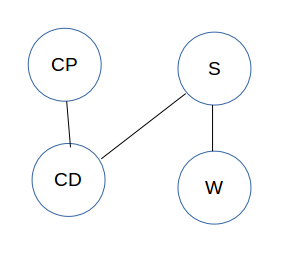
\includegraphics[keepaspectratio=true,scale=0.75]{constraint-graph}
\end{figure}
Below is the search tree with backtracking, without forward checking.
\begin{gather*}
    D_{CP} = \{0, 5, 10, 15\}, D_{CD} = \{0, 5, 10, 15\}, D_{S} = \{0, 5, 10, 15\}, D_{W} = \{0, 5, 10, 15\} \\
    CP = 0 \\
    D_{CP} = \{0, 5, 10, 15\}, D_{CD} = \{10, 15\}, D_{S} = \{0, 5, 10, 15\}, D_{W} = \{10, 15\} \\
    CP = 0, CD = 10 \\
    D_{CP} = \{0\}, D_{CD} = \{10, 15\}, D_{S} = \{0, 5, 10, 15\}, D_{W} = \{10, 15\} \\
    CP = 0, CD = 10, S = 0 \\
    D_{CP} = \{0\}, D_{CD} = \{10, 15\}, D_{S} = \{0\}, D_{W} = \{10, 15\} \\
    CP = 0, CD = 10, S = 0, W = 10
\end{gather*}
Finally the search tree below has backtracking and forward checking.
\begin{gather*}
    D_{CP} = \{0, 5, 10, 15\}, D_{CD} = \{0, 5, 10, 15\}, D_{S} = \{0, 5, 10, 15\}, D_{W} = \{0, 5, 10, 15\} \\
    CP = 0 \\
    D_{CP} = \{0, 5, 10, 15\}, D_{CD} = \{10, 15\}, D_{S} = \{0, 5, 10, 15\}, D_{W} = \{10, 15\} \\
    CP = 0, CD = 10 \\
    D_{CP} = \{0\}, D_{CD} = \{10, 15\}, D_{S} = \{0, 5, 10, 15\}, D_{W} = \{10, 15\} \\
    CP = 0, CD = 10, S = 0 \\
    D_{CP} = \{0\}, D_{CD} = \{10, 15\}, D_{S} = \{0\}, D_{W} = \{10, 15\} \\
    CP = 0, CD = 10, S = 0, W = 10
\end{gather*}
The search tree is identical because the order in which variables are assigned happened to be quite convenient.

\section{Appendix}
\begin{figure}[h]
\centering
\caption{Hill Climbing Figure}
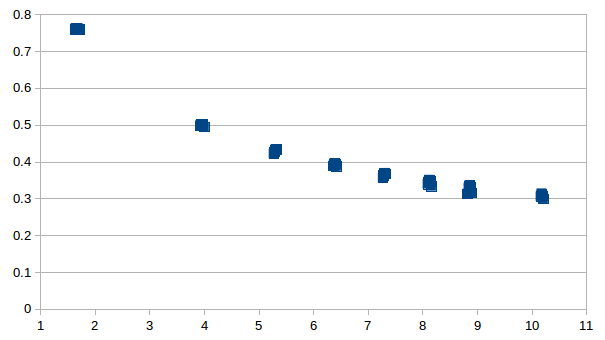
\includegraphics[keepaspectratio=true, scale=0.75]{hill-climbing}
\end{figure}
\par
\par
\begin{figure}[h]
\centering
\caption{Simulated Annealing Figure}
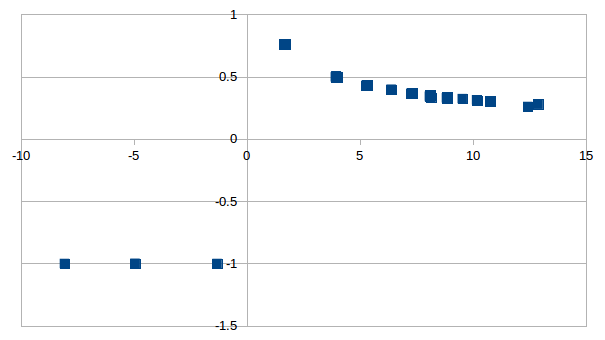
\includegraphics[keepaspectratio=true, scale=0.75]{simulated-annealing}
\end{figure}
\par
\par
\subsection{Hill Climbing Table}
X position, height, depth of search
\csvautolongtable{hillclimbing.csv}

\subsection{Simulated Annealing Table}
X position, height, depth of search
\csvautolongtable{simulatedannealing.csv}

\end{document}
